\documentclass[a4paper, letterpaper]{report}
\usepackage[french]{babel}
\usepackage[utf8]{inputenc}
\usepackage[T1]{fontenc}
\usepackage[pdftex]{graphicx}

%% Vervatim
\usepackage{verbatim}
\usepackage{fancyvrb}
%% listings
\usepackage{listings}
%% define color
\usepackage{xcolor}
\definecolor{codegreen}{rgb}{0,0.6,0}
\definecolor{codegray}{rgb}{0.5,0.5,0.5}
\definecolor{codepurple}{rgb}{0.58,0.0,82}
\definecolor{backcolour}{rgb}{0.95,0.95,0.92}

%% Python style
\lstdefinestyle{Pythonstyle}{
    language=Python, % programming language
    backgroundcolor=\color{backcolour},
    commentstyle=\color{codegreen},
    keywordstyle=\color{magenta},
    numberstyle=\tiny\color{codegray},
    stringstyle=\color{codepurple},
    basicstyle=\ttfamily\footnotesize,
    breakatwhitespace=false,
    breaklines=true,
    captionpos=b,
    keepspaces=true,
    numbers=left,
    numbersep=5pt,
    showspaces=false,
    showstringspaces=flase,
    showtabs=false,
    tabsize=2
}

\begin{document}

\begin{center}
    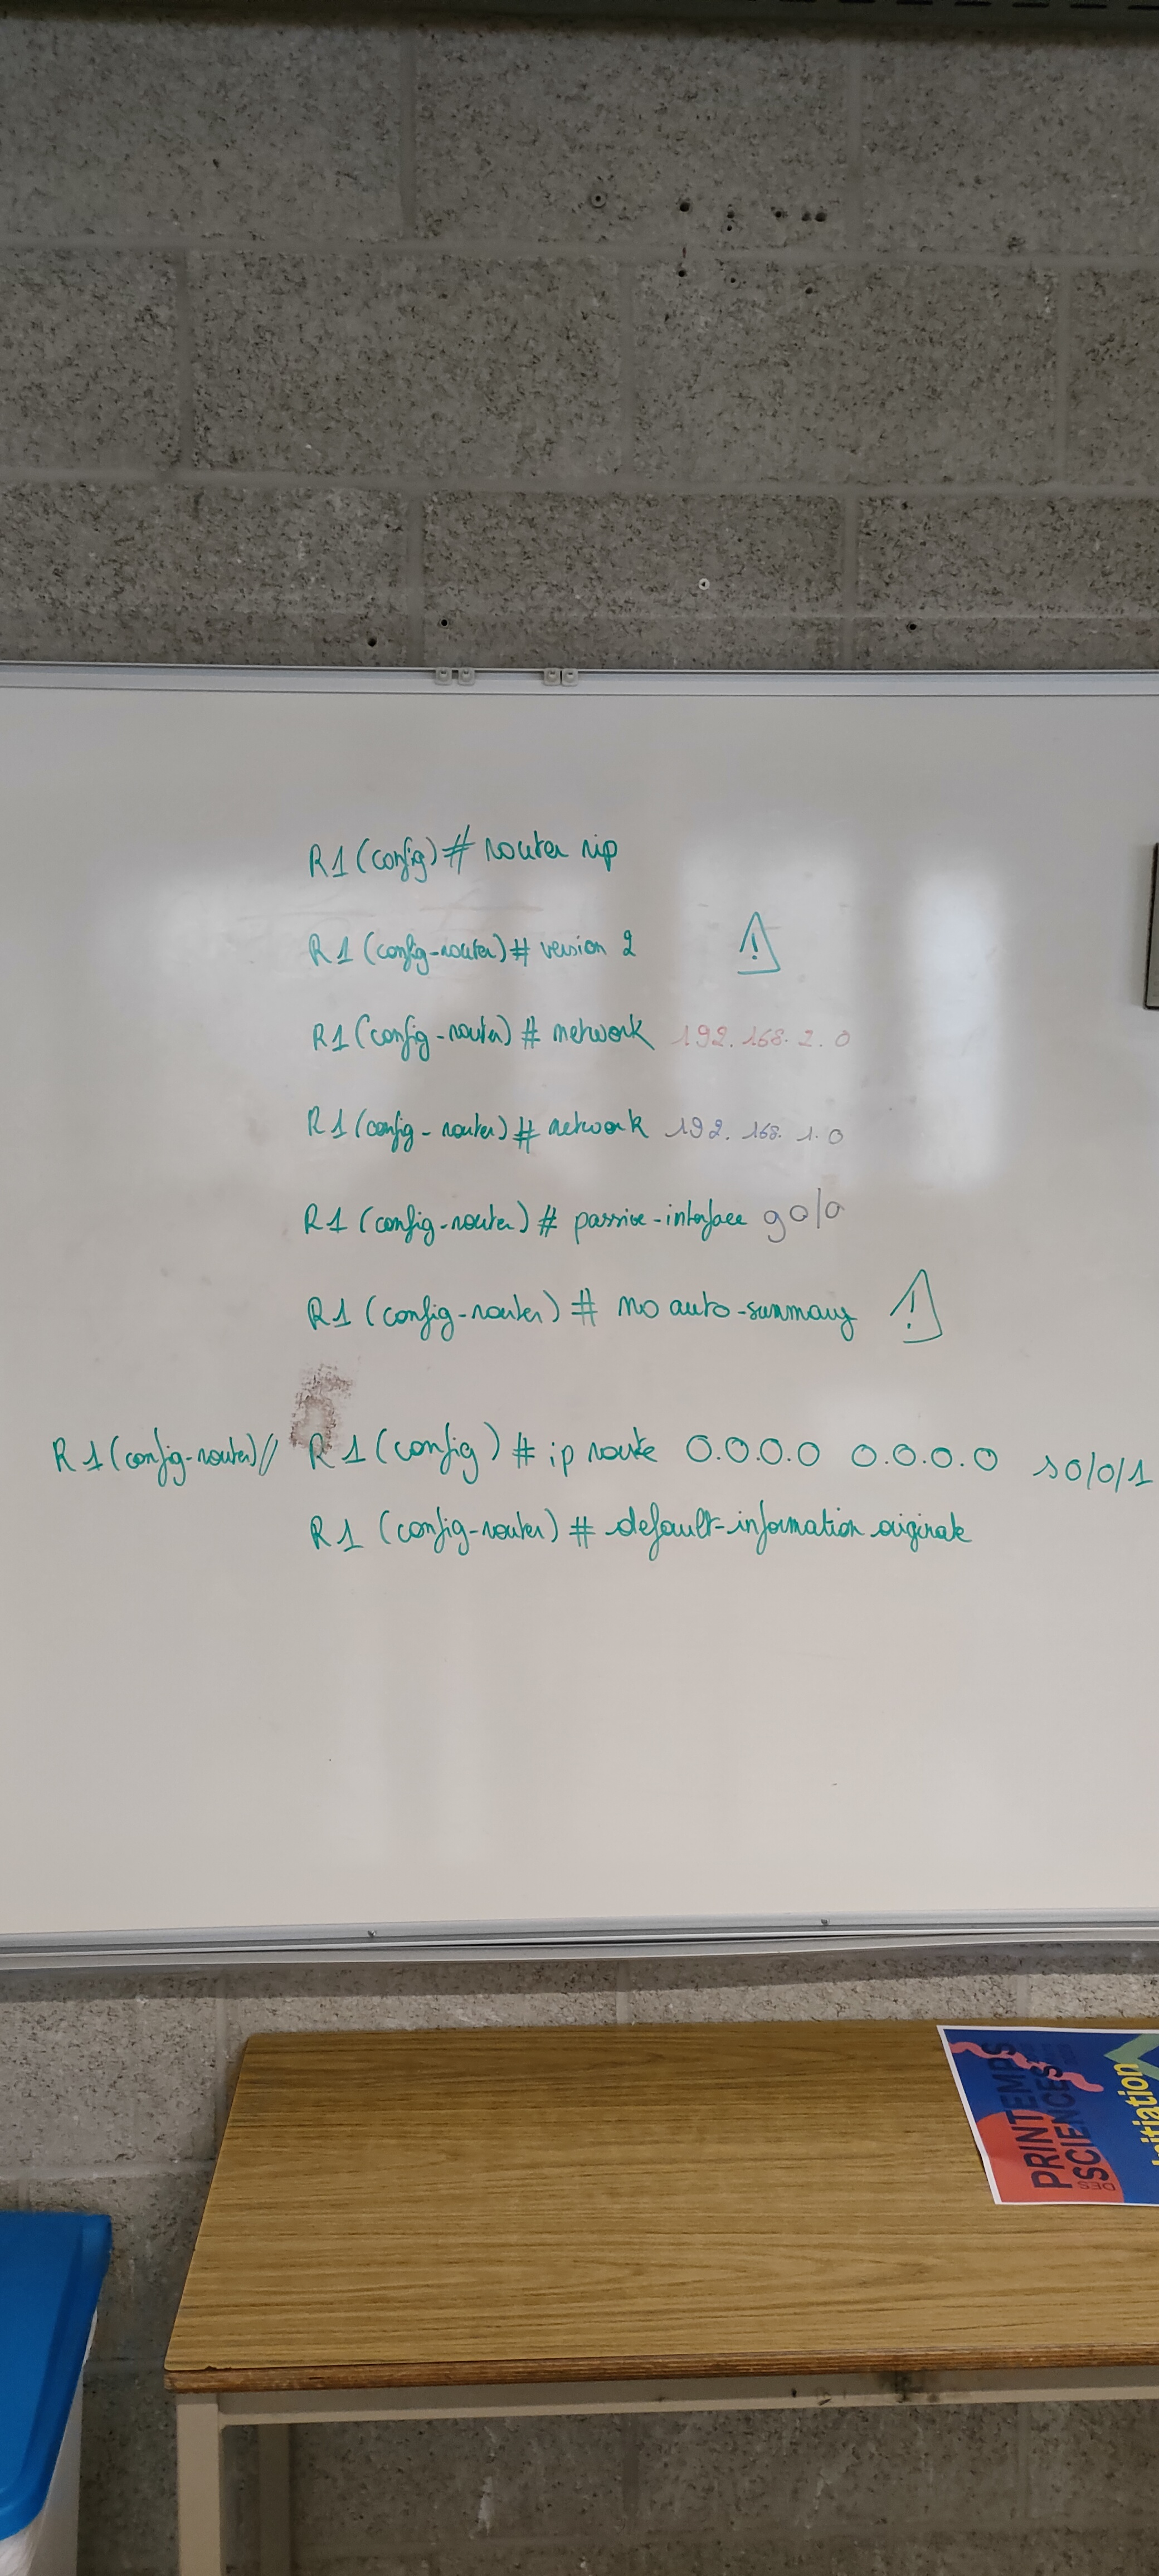
\includegraphics[scale=0.1]{IMG20230328093527.jpg}
\end{center}

\section{Python test}
\label{ss:python}

\begin{lstlisting}[style=Pythonstyle]
    # -*- coding: utf-8 -*-
"""
Created on Sat Mar  7 15:09:03 2020

@author: anne smal
"""
import random 
import datetime

class Human :
  
    def __init__ (self, name, bd=None) :
        self._name = name
        if bd :
            self._birthday = bd
        else :
            self._birthday = datetime.date.today()
        self._gender = random.choice('MF')

    @property
    def name(self):
        return self._name
    @name.setter
    def name(self, new_name):
        self._name = new_name
        
    """
    @property
    def age(self):
        return self._age
    @age.setter
    def age(self, new_age):
        self._age = new_age
    """
    
    @property
    def gender(self):
        return self._gender
    @gender.setter
    def gender(self, new_gender):
        self._gender = new_gender
        
    @property
    def birthday(self):
        return self._birthday
    
    def say(self, message) :
        print(self._name, ":", message)
        
        

    
    @property
    def age(self):
        today = datetime.datetime.now()
        age = today.year - self._birthday.year
        
        if (today.month<self._birthday.month) or (today.month == self._birthday.month and today.day<self._birthday.day):
            age -= 1
            
        return age    
        
        
if __name__=="__main__" :
    bd = datetime.date(2000, 2, 21)
    bob = Human("Bob",bd)    
    bob.say("I am " + str(bob.age) + " years old")
\end{lstlisting}

\end{document}